%!TEX root = widefieldscan.tex
\svnidlong
{$HeadURL$}
{$LastChangedDate$}
{$LastChangedRevision$}
{$LastChangedBy$}

\begin{center}
	\fbox{
		\begin{minipage}{.618\textwidth}
		The file of this section is \url{\svnkw{HeadURL}}, was last changed at: \svnfileday.\svnfilemonth.\svnfileyear \space \svnfilehour:\svnfileminute \space (UTC\svnfiletimezone) and is at revision \svnkw{LastChangedRevision}.
		\end{minipage}
	} 
\end{center}

\section{Results}
\label{sec:Results}
\subsection{Error between protocols}
A sequence of 19 protocols with varying quality has been scanned to assess the simulations. The properties of the scan have been chosen with according to a MATLAB-plot---as described in section~\ref{seq:Image Acquisition}---which has been generated with \verb+MATLAB\wfs-sim\main.m+ for a protocol with the diameter of \SI{3.8}{mm} and three overlapping subscans.

We assessed the image differences for the 19 scanned protocols in such a way that we have thresholded the raw data slices using an automated thresholding algorithm method, which chooses the threshold to minimize the intraclass variance of the black and white pixels~\cite{Otsu1979}. These thresholded slices of each protocol have been compared to the gold standard protocol in such a way that the sum of all pixels of the absolute difference image of the relevant protocol with the gold standard protocol has been taken and this difference image has been summed up to yield an error value. This error value has been calculated for 205 regularly spaced slices of the full dataset (1024 slices). The mean and standard deviation have been plotted (shown in figure~\ref{fig:NormalizedErrorPlot}) in such a way that the error in arbitrary units was scaled from 0 to 1.

We see that---as expected---the normalized error grows with decreasing amount of total obtained projections.\todo{explain some more!!!}

\begin{figure}
	\centering
		%\documentclass{article}
%\usepackage{tikz,pgfplots}
%\usepackage[pdftex,active,tightpage]{preview}
%\begin{document}
%\begin{preview}

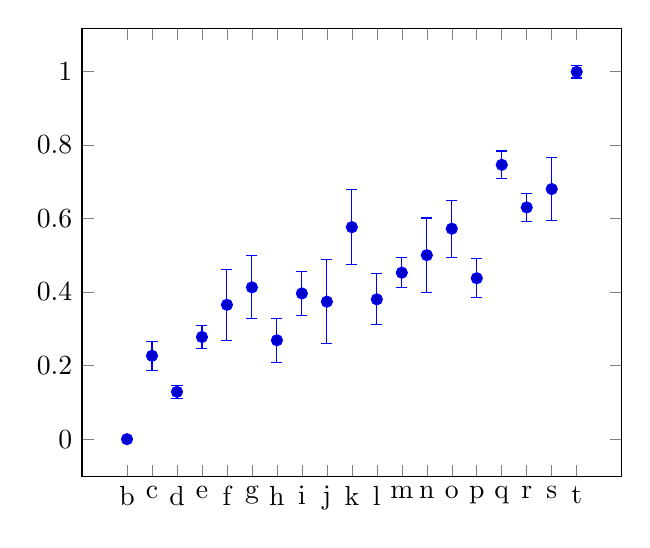
\begin{tikzpicture}
\begin{axis}[%
	%grid=both,%
	%xmajorgrids,%
	xtick={1,2,3,4,5,6,7,8,9,10,11,12,13,14,15,16,17,18,19},%
	xticklabels={b,c,d,e,f,g,h,i,j,k,l,m,n,o,p,q,r,s,t},%
]
% Line plot
\addplot
	plot[ 	%smooth,
	   		only marks,
	      	error bars/.cd,
	      	y dir=both, y explicit %
		]
	coordinates{
	(1,0) 			+- (0,0)
	(2,0.226697)	+- (0,0.0389)
	(3,0.128649)	+- (0,0.0174)
	(4,0.277819)	+- (0,0.0316)
	(5,0.365309) 	+- (0,0.0960)
	(6,0.412726)	+- (0,0.0856)
	(7,0.268849) 	+- (0,0.0598)
	(8,0.396237)	+- (0,0.0589)
	(9,0.373823)	+- (0,0.1148)
	(10,0.576375)	+- (0,0.1020)
	(11,0.380172) 	+- (0,0.0696)
	(12,0.452672)	+- (0,0.0404)
	(13,0.500303)	+- (0,0.1010)
	(14,0.572158)	+- (0,0.0778)
	(15,0.437586)	+- (0,0.0524)
	(16,0.745885)	+- (0,0.0376)
	(17,0.630023)	+- (0,0.0386)
	(18,0.679989)	+- (0,0.0852)
	(19,0.998734)	+- (0,0.0169)
};

\end{axis}
\end{tikzpicture}


% plot erstellt mit MATLAB-File p:\doc\MATLAB\WFS-CompareDMPs\wfs_Compare2008c.m (FromToTo = 1:5:1024)
% und matlab2tikz

%[ 1:19;std(NormCumulativeError);mean(NormCumulativeError)]
%
%ans =
%
%  Columns 1 through 12
%
%    1.0000    2.0000    3.0000    4.0000    5.0000    6.0000    7.0000    8.0000    9.0000   10.0000   11.0000   12.0000
%         0    0.0389    0.0174    0.0316    0.0960    0.0856    0.0598    0.0589    0.1148    0.1020    0.0696    0.0404
%         0    0.2267    0.1286    0.2778    0.3653    0.4127    0.2688    0.3962    0.3738    0.5764    0.3802    0.4527
%
%  Columns 13 through 19
%
%   13.0000   14.0000   15.0000   16.0000   17.0000   18.0000   19.0000
%    0.1010    0.0778    0.0524    0.0376    0.0386    0.0852    0.0169
%    0.5003    0.5722    0.4376    0.7459    0.6300    0.6800    0.9987          	
         	
%
%\end{preview}
%\end{document}
	\caption{Plot of normalized Error for the different protocols. The normalized Error has been calculated in such a way that we have taken the DifferenceImage for Protocol 'x' compared to Protocol 'A' and . The error bars for each protocol show the standard deviation of the error which was calculated for 205 of the 1024 slices for each protocol.}
	\label{fig:NormalizedErrorPlot}
\end{figure}

\subsection{Image Merging and Reconstruction}
Results of the steps mentioned in section~\ref{sec:materials and methods} are shown in figure~\ref{fig:wide field scan results}. Figure~\ref{fig:subscans} shows exemplary projection images from overlapping subscans prior to correction and normalization. Figure~\ref{fig:merge-proj} shows a merged projection image prior to reconstruction and figure~\ref{fig:merge-rec} shows the end-result of such a wide field scan, a reconstructed slice of the whole sample with a FOV of \SI{5.734}{\milli\meter} which is approximately three times the size of what can be achieved with one single scan.

\begin{figure}[p]
	\renewcommand{\imsize}{.16\linewidth}
	\pgfmathsetlength{\imagewidth}{\imsize} % desired display width of image
	\pgfmathsetlength{\imagescale}{\imagewidth/512} % pixel width of image
	\centering
		\subfloat[Uncorrected projection images from subscans s$_1$--s$_3$, each with a size of 1024$\times$1024 pixels at a resolution of \SI{1.4}{\micro\meter\per pixel}, covering a FOV of approximately \SI{0.7}{\milli\meter}. The scans overlap each other by approximately 100 pixels. 4676 projections have been acquired for the subscans s$_1$ and s$_3$, 1169 projections have been acquired for subscan s$_2$, all over a rotation of \SI{180}{\degree}.]{%
			\label{fig:s1}%
			\includegraphics[width=\imsize]{img/merge/R108C10B-s1}%
			\includegraphics[width=\imsize]{img/merge/R108C10B-s2}%
			\begin{tikzpicture}[x=\imagescale,y=-\imagescale]
				% place image (integer coordinates refer to pixel centers):
				\node[anchor=north west,inner sep=0pt,outer sep=0pt] at (0,0)
					{\includegraphics[width=\imagewidth]{img/merge/R108C10B-s3}};
				\draw[|-|,color=white] (256-64,450) -- (512-64,450) node[midway,above] {\SI{700}{\micro\meter}};
			\end{tikzpicture}
			\label{fig:subscans}
			}
		\renewcommand{\imsize}{.48\linewidth}
		\pgfmathsetlength{\imagewidth}{\imsize} % desired displayed width of image
		\pgfmathsetlength{\imagescale}{\imagewidth/1498} % pixel width of image
		\subfloat[Merged and corrected image from the three subscans shown in subfigure~\subref{fig:subscans}. The merged projections have a size of 2994$\times$1024 pixels at a resolution of \SI{1.4}{\micro\meter\per pixel}. The Subscans s$_1$--s$_3$ overlap each other by approximately 150 pixels, thus the width of the merged projection is smaller than three times the width of the subscans. The projections of the subscans above have been merged into 4676 projections images like the one shown here and were then reconstructed into a tomographic dataset using a filtered backprojection reconstruction algorithm.]{%
			\begin{tikzpicture}[x=\imagescale,y=-\imagescale]
				\node[anchor=north west,inner sep=0pt,outer sep=0pt] at (0,0)
					{\includegraphics[width=\imagewidth]{img/merge/R108C10B-merge}};
				\draw[|-|,color=white] (1242-64,450) -- (1498-64,450) node[midway,above] {\SI{700}{\micro\meter}};
			\end{tikzpicture}
			\label{fig:merge-proj}
			}
		\renewcommand{\imsize}{\linewidth}
		\pgfmathsetlength{\imagewidth}{\imsize} % desired displayed width of image
		\pgfmathsetlength{\imagescale}{\imagewidth/1365} % pixel width of image (image has been resized from 2994*1123, so that scalebar is at the same height without calculating too much...)
		\subfloat[Cropped part of one slice of the tomographic dataset reconstructed from the merged projections, where one is shown in subfigure~\subref{fig:merge-proj}. The halo directly around the lung tissue arises from the paraffin where the sample is embedded in. The bright circular shape inscribed in the square arises from the filtered backprojection, the chosen reconstruction method. The size of the cropped image is 2994$\times$1123 pixels. The small inset on the upper left corner shows an overview over the full slice with a size of 2994$\times$2994 pixels.]{%
			\begin{tikzpicture}[x=\imagescale,y=-\imagescale]
				% place image (integer coordinates refer to pixel centers):
				\node[anchor=north west,inner sep=0pt,outer sep=0pt] at (0,0)
					{\includegraphics[width=\imagewidth]{img/merge/R108C10B-merge1016-crop}};
				\newcommand{\size}{.2\imagewidth}
				\node[anchor=north west,inner sep=0pt,outer sep=0pt] at (0,0)
					{\includegraphics[width=\size]{img/merge/R108C10B-merge1016}};
					\draw[white] (\size,0) -- (\size,-\size) -- (0,-\size);
				\draw[|-|,color=white] (1109-64,450) -- (1365-64,450) node[midway,above] {\SI{700}{\micro\meter}};
			\end{tikzpicture}
			\label{fig:merge-rec}
			}
	\caption{Different stages of a wide field scan of a rat lung sample obtained from a Sprague-Dawley rat 10 days after birth, showing the distal-medial edge of the right lower lung lobe. The sample has been scanned at a beam energy of \SI{12.6}{\kilo\electronvolt}.}
	\label{fig:wide field scan results}	
\end{figure}

\subsection{Three dimensional visualizations}
\subsubsection{19 Protocols}
\begin{figure}
	\centering
	\renewcommand{\imsize}{.5\linewidth}	
		\subfloat[Overview Protocol B]{%
			\includegraphics[width=\imsize]{img/protocols/BvsT/overviewB}}
		\subfloat[Overview Protocol T]{%
			\includegraphics[width=\imsize]{img/protocols/BvsT/overviewT}}\\
	\renewcommand{\imsize}{.495\linewidth}
		\subfloat[Detailed view of segments of Protocol B]{%
			\includegraphics[width=\imsize]{img/protocols/BvsT/detail-1-B}}\hfill
		\subfloat[Detailed view of segments of Protocol B]{%
			\includegraphics[width=\imsize]{img/protocols/BvsT/detail-1-T}}\\
		\subfloat[Detailed view of underside of Protocol B]{%
			\includegraphics[width=\imsize]{img/protocols/BvsT/detail-2-B}}\hfill
		\subfloat[Detailed view of underside of Protocol T]{%
			\includegraphics[width=\imsize]{img/protocols/BvsT/detail-2-T}}
	\caption{Segmentation of two exemplary protocols, namely B and T.}
	\label{fig:BvsT}
\end{figure}

\subsubsection{5 instead of 3 subscans}
\begin{figure}[p]
	\renewcommand{\imsize}{\linewidth}
	\pgfmathsetlength{\imagewidth}{\imsize} 		 % desired displayed width of image
	\pgfmathsetlength{\imagescale}{\imagewidth/1589} % 1589*728 = width of imagefile used below
	\newcommand{\startx}{982} %= 1589*.618
	\newcommand{\starty}{655} %= 728*.9
	\centering
	\subfloat[]{
		\begin{tikzpicture}[x=\imagescale,y=-\imagescale]
 			\node[anchor=north west,inner sep=0pt,outer sep=0pt] at (0,0)
 			{\includegraphics[width=\imagewidth]{img/sophie/full}};
 			\draw[|-|](\startx-808,\starty) -- (\startx+500,\starty) node[midway,above] {\SI{3.3978}{\milli\meter}}; % 4854px * 0.7 um/px = 3.3978 mm
	 	\end{tikzpicture}
	 	\label{subfig:LungSlab}
		}
	\renewcommand{\imsize}{.25\linewidth}
	\pgfmathsetlength{\imagewidth}{\imsize} % desired displayed width of image
	\pgfmathsetlength{\imagescale}{\imagewidth/902} % 1543*928 = width of imagefile used below
	\renewcommand{\startx}{557} %= 902*.618
	\renewcommand{\starty}{802} %= 891*.9
	\subfloat[]{%
		\begin{tikzpicture}[x=\imagescale,y=-\imagescale]
			\node[anchor=north west,inner sep=0pt,outer sep=0pt] at (0,0)
 			{\includegraphics[width=\imagewidth]{img/sophie/crop-green-background}};
 			\draw[|-|] (\startx+0,\starty) -- (\startx+200,\starty) node[midway,above] {\SI{179.2}{\micro\meter}}; % cube with 256 px = 179.2 um
	 	\end{tikzpicture}%
	 	\label{subfig:LungSlabDetailsGreenBG}%
		}
	\subfloat[]{%
		\begin{tikzpicture}[x=\imagescale,y=-\imagescale]
			\node[anchor=north west,inner sep=0pt,outer sep=0pt] at (0,0)
 			{\includegraphics[width=\imagewidth]{img/sophie/crop-green}};
 			\draw[|-|] (\startx+0,\starty) -- (\startx+200,\starty) node[midway,above] {\SI{179.2}{\micro\meter}}; % cube with 256 px = 179.2 um
	 	\end{tikzpicture}%
	 	\label{subfig:LungSlabDetailsGreen}%
		}%
	\subfloat[]{%
		\begin{tikzpicture}[x=\imagescale,y=-\imagescale]
			\node[anchor=north west,inner sep=0pt,outer sep=0pt] at (0,0)
 			{\includegraphics[width=\imagewidth]{img/sophie/crop-red}};
 			\draw[|-|] (\startx+0,\starty) -- (\startx+200,\starty) node[midway,above] {\SI{179.2}{\micro\meter}}; % cube with 256 px = 179.2 um
	 	\end{tikzpicture}%
	 	\label{subfig:LungSlabDetailsRed}%
		}
	\subfloat[]{%
		\begin{tikzpicture}[x=\imagescale,y=-\imagescale]
			\node[anchor=north west,inner sep=0pt,outer sep=0pt] at (0,0)
 			{\includegraphics[width=\imagewidth]{img/sophie/crop-red-background}};
 			\draw[|-|] (\startx+0,\starty) -- (\startx+200,\starty) node[midway,above] {\SI{179.2}{\micro\meter}}; % cube with 256 px = 179.2 um
	 	\end{tikzpicture}%
	 	\label{subfig:LungSlabDetailsRedBG}%
		}
	\caption{Visualization of lung tissue slab: %
		\subref{subfig:LungSlab}: Three dimensional volume rendering of slab of lung tissue with a size of 554$\times$4854$\times$1024 pixels at a voxel size of \SI{0.7}{\micro\meter} per pixel. Both inset cubes have a side length of 256 pixels and were automatically segmented using a region growing algorithm. 
 		\subref{subfig:LungSlabDetailsGreenBG}: Closeup of inset cube at an outer position in the sample, including the background tissue. % 
 		\subref{subfig:LungSlabDetailsGreen}: Closeup of inset cube at an outer position in the sample. Albeit we have been able to automatically segment the lung tissue, segmentation artifacts are visible. Single alveoli can be distinguished. %
 		\subref{subfig:LungSlabDetailsRed}: Closeup of inset cube at a central position in the sample. Single alveoly are clearly visible. %
 		\subref{subfig:LungSlabDetailsRedBG}: Closeup of inset cube at a central position in the sample, including the background tissue. %
		The scale bars are only approximate, since it is a three-dimensional view. The top scale bar is valid for the longest length of the gray lung structure, the bottom scale bar is valid for the width of the red cube.%
	}
	\label{fig:LungSlabSophie}
	\todo[inline]{adapt the scalebars to the final size of the images}
\end{figure}